


\documentclass[12pt]{report}
\usepackage[english]{babel}
\usepackage{amsmath}
\usepackage[utf8x]{inputenc}
\usepackage{amsmath}
\usepackage{graphicx}
\graphicspath{{.images/}}
\usepackage{parskip}
\usepackage{fancyhdr}
\usepackage{vmargin}
\setmarginsrb{3 cm}{2.5 cm}{3 cm}{2.5 cm}{1 cm}{1.5 cm}{1 cm}{1.5 cm}
\newcommand*{\hatH}{\hat{\mathcal{H}}}

\title{Quantum Dots}								
% Title
\author{ Kavi Chapagain}						
% Author

\makeatletter
\let\thetitle\@title
\let\theauthor\@author
\makeatother

\pagestyle{fancy}
\fancyhf{}
\rhead{\theauthor}
\lhead{\thetitle}
\cfoot{\thepage}
%%%%%%%%%%%%%%%%%%%%%%%%%%%%%%%%%%%%%%%%%%%%
\begin{document}

%%%%%%%%%%%%%%%%%%%%%%%%%%%%%%%%%%%%%%%%%%%%%%%%%%%%%%%%%%%%%%%%%%%%%%%%%%%%%%%%%%%%%%%%%

\begin{titlepage}
	\centering
    \vspace*{0.5 cm}
    
\begin{center}    \textsc{\Large   Modern Physics}\\[2.0 cm]	\end{center}
	\textsc{\Large PEN231  }\\[0.5 cm]				% Course Code
	\rule{\linewidth}{0.2 mm} \\[0.4 cm]
	{ \huge \bfseries \thetitle}\\
	\rule{\linewidth}{0.2 mm} \\[1.5 cm]
	
	\begin{minipage}{0.4\textwidth}
		\begin{flushleft} \large
			\end{flushleft}
			\end{minipage}~
			\begin{minipage}{0.4\textwidth}
			\begin{flushright} \large
			\emph{Submitted By :} \\Kavi Chapagain 
		\end{flushright}
	\end{minipage}\\[2 cm]
	
    
    
	
\end{titlepage}


\tableofcontents
\pagebreak


\renewcommand{\thesection}{\arabic{section}}
\section{Introduction}

Quantum Dots are the real world particle in a box. They are the nanoparticles in which a particular colour is observed when illuminated by the light. It has a lot of applications ranging from using in solar cells to the quantum screen used in computer/TV screens.
\newline In this experiment, we will experimentally determine the size of a Quantum Dot. First, an energy equation for a one-dimensional particle in a box is derived, then in the experimental section the size of the Quantum Dots is determined.


\section{Theory}
In 1925 Austrian Physicist Erwin Schrodinger introduced the wave equation, named after him Schrodinger Equation. The equation is:
\begin{equation}
    \hatH \Psi = E \Psi          
\end{equation}

Here, $\hatH$ is the Hamiltonian operator is the eigen value of the wave function$\psi$. The $\hatH$ can be expressed as:
\begin{equation}
    \hatH = - \frac{\hbar^2}{2m} \frac{\delta^2}{\delta x^2} + V(x)
\end{equation}
 From equation 1 and equation 2:
 \begin{equation}
    - \frac{\hbar^2}{2m} \frac{\delta^2 \Psi(x)}{\delta x^2} + V(x) = E \Psi(x)
 \end{equation}
First we will derive the energy for one dimensional particle in a box then derive three dimensional later. Since the potential inside the well is zero, the Equation 3 can be simplified as:
\begin{equation}
     - \frac{\hbar^2}{2m} \frac{\delta^2 \Psi(x)}{\delta x^2} = E \Psi(x)
\end{equation}
Rearranging Equation 4,
\begin{equation}
    \frac{\delta^2 \Psi(x)}{\delta x^2} =  - \frac{2mE}{\hbar^2} \Psi(x)
\end{equation}
Define a variable $k^2$:
\begin{equation}
    k^2 = \frac{2mE}{\hbar}
\end{equation}
Now, the Shrondinger Equation is further simplified as:
\begin{equation}
    \frac{\delta^2 \Psi(x)}{\delta x^2} =  -k^2 \Psi(x)
\end{equation}
The general solution of this differential equation is
\begin{equation}
    \Psi(x) = Asin(kx) + Bcos(kx)
\end{equation}
and,
\begin{equation}
      E = \frac{k^\hbar}{2m}
\end{equation}

The potential outside the box is infinite, the wave function should be 0 at the edge of the box. 
\begin{equation}
    \Psi(0) = \Psi(L) = 0
\end{equation}

So, when x=0,
\begin{equation}
    \Psi(0) = Asin(0) + Bcos(0) = A.0 + B.1 = 0
\end{equation}
This means the value of B is 0 at the boundary. So, our wave function becomes
\begin{equation}
    \Psi(x) = Asin(kx)
\end{equation}
Now, when x=L,
\begin{equation}
    \Psi(L) = Asin(kL) = 0
\end{equation}
The Equation 12 implies
\begin{equation}
    kL = \pi, 2\pi, 3\pi, ...
\end{equation}
which means
\begin{equation}
    k = \frac{n\pi}{L}, n=1, 2, 3, ...
\end{equation}
From Equation 10 and Equation 14, the wave function is:
\begin{equation}
    \Psi_n(x) = Asin(\frac{n\pi x}{L})
\end{equation}
and
\begin{equation}
    E_n = \frac{n^2\pi^2\hbar^2}{2mL^2}
\end{equation}
This is for the one dimensional square shape particle. \newpage 
For the three dimensional and spherical particle which is the shape of the Quantum Dots used in this experiment. The lowest energy state is given by 

\begin{equation}
    E_{sphere} = \frac{\hbar^2 \pi^2}{2mR^2},
\end{equation}
where R is the radius of the Quantum Dot
\newline
There are two particles, the electron and the hole, so the energy is
\begin{equation}
    E_{sphere} = \frac{\hbar^2 \pi^2}{2m_eR^2} + \frac{\hbar^2 \pi^2}{2m_hR^2}, \label{eq: 3d-qd}
\end{equation}
In the Equation \eqref{eq: 3d-qd}, $m_e$ is the mass of the electron, $m_h$ is the mass of the hole inside the semiconductor and R is the radius of the Quantum Dot.
\newline
The Quantum Dot box is filled with a semiconductor. Taking that in account, the energy of semiconductor band gap ($E_g$) is added our base-line energy. Therefore, 
\begin{equation}
     E_{sphere} = \frac{\hbar^2 \pi^2}{2m_eR^2} + \frac{\hbar^2 \pi^2}{2m_hR^2} + E_g 
\end{equation}
The following values are available:
\newline
$E_g = 2.15 \times 10^-19$ J
\newline
$m_e = 7.29 \times 10^-32$ kg
\newline
$m_h = 5.47 \times 10^-31$ kg

Similarly, in the experiment, the wavelength of the light from the Quantum Dots is measured and the zero-point energy is calculated by using
\begin{equation}
    E = hf \: and \: f = \frac{c}{\lambda}
\end{equation}
where E, h, f, c and $\lambda$ are is the energy, Plank's constant(6.625$\times 10^-34$Js), frequency, speed of the light (3.0$\times 10^8$m/s) and the wavelength respectively.


\section{Experiment}

The experiment is conducted to determine the radii of four different size of Quantum Dots. The four quantum dots were in a  solution of a different colour, red, orange, yellow and green. A clamp was set to hold the solution and was exposed with 400nm LED light. Then the data was collected by using a spectrometer sensor and a computer program Data Logger. The wavelength of the four solutions is shown in the Table \ref{tbl:wl}.
\newline

\begin{table}[]
\centering
\begin{tabular}{|c|c|c|}
\hline
\textbf{\#} & \textbf{Colour} & \textbf{$\lambda(nm)$} \\ \hline
1          & Red             & 624.7                  \\ \hline
2          & Orange          & 592.2                  \\ \hline
3          & Yellow          & 565.7                  \\ \hline
4          & Green           & 537.1                  \\ \hline
\end{tabular}
\caption{Experimentally Recorded Wavelength of Each Solution }
\label{tbl:wl}
\end{table}


\section{Analysis}


The energy of the quantum dots is given by Equation 21 and Equation 20, combining both we get
\begin{equation}
    E = \frac{\hbar^2 \pi^2}{2m_eR^2} + \frac{\hbar^2 \pi^2}{2m_hR^2} + E_g 
\end{equation}
or,
\begin{equation*}
    E - E_g  = \frac{\hbar^2 \pi^2}{2R^2} (\frac{1}{m_e} + \frac{1}{m_h}) 
\end{equation*}
\begin{equation*}
    R^2 =   \frac{\hbar^2 \pi^2}{2} (\frac{1}{m_e} + \frac{1}{m_h}) \times \frac{1}{E - E_g}
\end{equation*}
Substituting the values of $\hbar,$ $\pi,$ $m_e$, and  $m_h$, we get
\begin{equation}
    R =   9.20\times  10^{-19} \sqrt{\frac{1}{\frac{hc}{\lambda} - E_g}}
\end{equation}

So, the calculated values of the experimental radius of quantum dots from the Equation 23 is shown in Table \ref{tbl:radius}.

\begin{table}[]
\centering
\begin{tabular}{|c|c|c|l|}
\hline
\textbf{\#} & \textbf{Colour} & \textbf{Radius (nm)}  \\ \hline
1          & Red             & 2.86                   \\ \hline
2          & Orange          & 2.64                \\ \hline
3          & Yellow          & 2.49                \\ \hline
4          & Green           & 2.33                 \\ \hline
\end{tabular}
\caption{Calculated Radius and Percentage Uncertainty }
\label{tbl:radius}
\end{table}

The accepted value with the percentage uncertainty is shown in the Table \ref{tbl:uncertain}. The experimental value is 1-3\% variant from the accepted radius.

\begin{table}[]
\centering
\begin{tabular}{|c|c|c|l|l|}
\hline
\textbf{\#} & \textbf{Colour} & \textbf{\begin{tabular}[c]{@{}c@{}}Experimental\\ Radius (nm)\end{tabular}} & \textbf{\begin{tabular}[c]{@{}l@{}}Accepted \\ Radius (nm)\end{tabular}} & \textbf{\begin{tabular}[c]{@{}l@{}}Percentage \\ Error (\%)\end{tabular}} \\ \hline
1           & Red             & 2.86                                                                          & 2.92                                                                        & 2.05                                                                           \\ \hline
2           & Orange          & 2.64                                                                       & 2.71                                                                        & 2.58                                                                           \\ \hline
3           & Yellow          & 2.49                                                                       & 2.53                                                                        & 1.58                                                                           \\ \hline
4           & Green           & 2.33                                                                       & 2.37                                                                        & 1.69                                                                           \\ \hline
\end{tabular}
\caption{Accepted Value and Percentage Error }
\label{tbl:uncertain}
\end{table}

The plot of quantum dot radius vs. the emitted wavelength is shown in Fig \ref{fig:qd_plot}. It shows the radius of a quantum dot is directly proportional to the emitted wavelength and tries to show a linear relationship. The gradient of 0.006 is also observed, which is seen as a gradual positive increment of the radius with respect to wavelength in the graph.

\begin{figure}
    \centering
    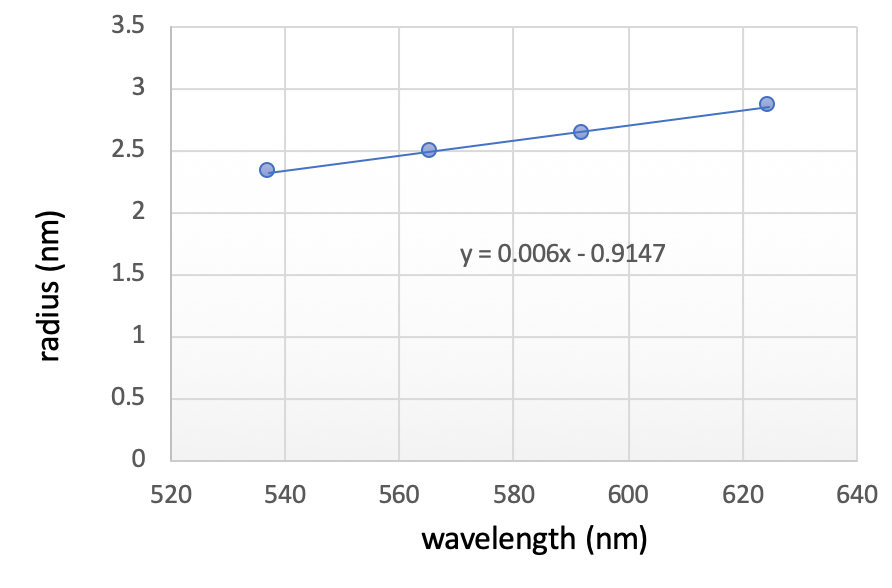
\includegraphics[width=0.65\textwidth] {images/r-w}
    \caption{Quantum dot radius vs. Emitted wavelength}
    \label{fig:qd_plot}
\end{figure}
    
\section{Conclusion}
In this experiment, we determined the size of a Quantum Dot using the wavelength emitted by the containing solution. The values recorded are shown in Table \ref{tbl:wl}. The percent error between the experimental radius and the accepted radius was less than 2.60\%.  \\
The noise on the data can be reduced by conducting the experiment in a dark room, switching off the lights.

 
\begin{thebibliography}{9}
   
  
\bibitem{b1} 
   Experiment Guide, Operating Instructions: 1751-18 CENCO Quantum Dots, Nanosys

\end{thebibliography}
\end{document}

